\chapter{SegRanks: Manual Evaluation Based on Short Segments}
\label{chapter:segranks}

In the following two chapters, we propose a novel manual evaluation method in
which we create a database of human annotations. This database could be reused
later to automatically evaluate similar but unseen translations or even
to tune systems.  This method therefore lies on the boundary of automatic and
manual evaluation methods.

The proposed method consists of two parts, which we describe and experiment
with in the following two chapters. In this chapter, we describe the way of
collecting the database of human judgements and report the human annotation
experiment which we conducted using the proposed method. In the following
chapter, we present some methods which exploit the collected database: besides
the evaluation of annotated systems, we experiment with extrapolating the
database to evaluate unseen translations and with tuning a machine translation
system using the database.

In the WMT official human evaluation, humans judge whole sentences. They get
five candidate translations of a given source sentence and their task is to
rank these candidates relatively to one another (ties are allowed). One of
the disadvantages of this method is that the sentences are quite long and therefore
quite hard to remember for the judge to compare them. Also, when comparing
longer sentences, there are many more aspects in which one sentence can be
better or worse than another, and therefore it is more difficult for
judges to choose the better of the candidates. 

\begin{algorithm}
    \begin{algorithmic}[1]
        %\Require{$x$ and $y$ are packed DNA strings of equal length $n$}
        \Function{ExtractSegments}{$treeNode, minLength, maxLength$}
            \Let{$extractedSegments$}{$list()$}
            \Let{$leaves$}{$treeNode.leaves()$}
            \If{$length(leaves) \le maxLength$}
                \If{$lenth(leaves) \ge minLength$}
                    \State $extractedSegments.append(leaves)$
                \EndIf
            \Else
                \For{$node$ \textbf{in} $treeNode.children()$  }
                \Let{$segments$}{\textsc{ExtractSegments}$(child, minLength, maxLength))$}
                \State $extractedSegments.extend(segments)$
                \EndFor
            \EndIf
            \Return $extractedSegments$
        \EndFunction
    \end{algorithmic}
    \caption{Short Segment Extraction From Source Side Parse Tree}
    \label{segment:extraction}
\end{algorithm}

To avoid these disadvantages, we propose the following method. Instead of
judging whole sentences, we extract short segments\footnote{The term `segment'
is sometimes used in the literature to refer a sentence. In this thesis, we
will use the term `segment' for a phrase of few words. } from candidates and
give them to judges to rank them. In order to extract meaningful segments with
the same meaning from all candidates, we do the following procedure: First, we
parse the source sentence and then recursively descend the parsed tree and find
nodes which cover source segments of a given maximum length. This is described
exactly in Algorithm \ref{segment:extraction}. Finally, we project these
extracted source segments to their counterpart segments in all candidate
sentences using an automatic alignment.  You can find the whole process
illustrated in Figure \ref{tree-align}. This extraction method is inspired by
\perscite{human-in-the-loop} and by the WMT07 manual evaluation
\parcite{wmt-overview-2007}.


In the segment evaluation in \parcite{wmt-overview-2007}, these extracted
segments are only highlighted and shown to judges together with the rest of the
sentence.  Judges are asked to rank the highlighted segments in the context of the
whole candidate sentences.

We use a different approach here which is more similar to that used by
\perscite{human-in-the-loop}. We show the extracted segments without any context
and ask judges to rank them. The only additional information provided to
annotators is the whole source sentence with the source segment highlighted.
Judges are told that they can imagine the rest of the sentence in which the
ranked segment fits best. They are instructed to penalize only those segments
for which they cannot imagine any appropriate rest of the sentence.

While we are aware that this approach has some disadvantages (which we
summarize below) there is one significant advantage: it is much more likely
that two systems produce the same translation of a short segment than that they
would produce the same translation of a whole sentence. Because we do not show
the sentence context to annotators, we can merge identical segment candidates
into one, so the annotators have fewer candidate segments to rank. This also
allows us to reuse already collected human judgements later to evaluate a new
system which was not in the set of annotated systems or to tune parameters of a
system.

\begin{figure}
    \begin{center}
        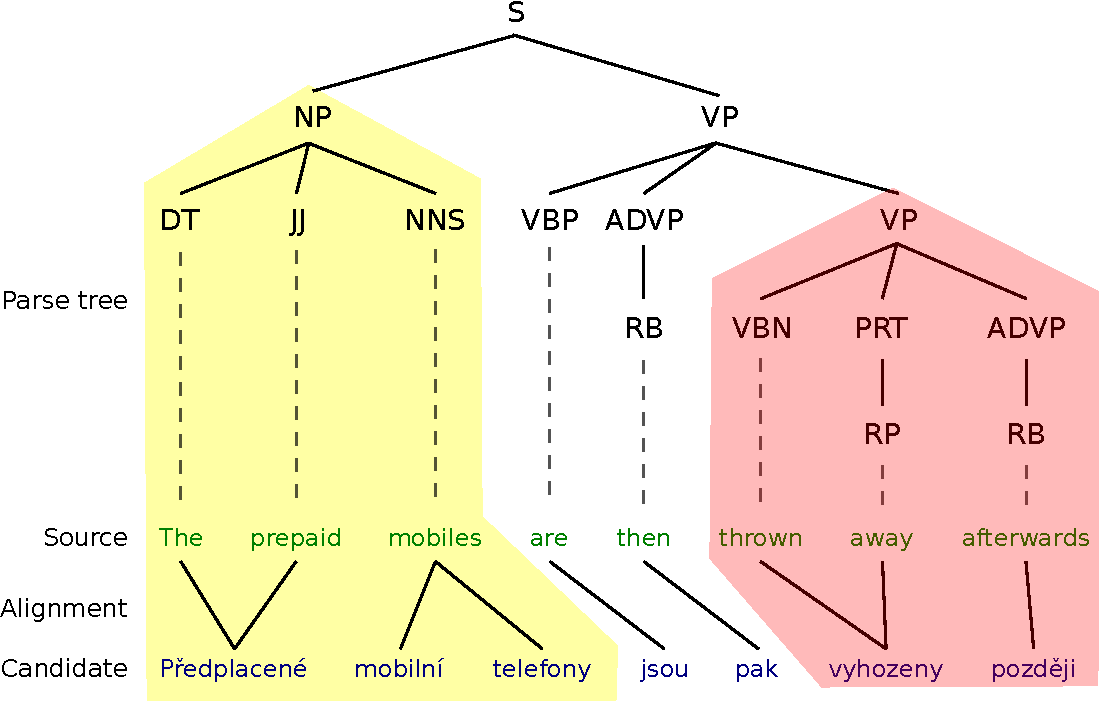
\includegraphics[width=\textwidth]{img/tree-align.pdf}
    \end{center}

    \caption[An illustration of the candidate segments extraction process]{ An
      illustration of candidate segments extraction process. For a given MT
      system, two segments were extracted from this sentence. The
      \pojem{maxLength} constant was set to the value 4 here, to illustrate that
      not all of the words are always covered by the extracted segments.

}
    \label{tree-align}
\end{figure}

The following list summarizes disadvantages of this method, which we are aware
of. However, we believe that the advantages still outweight the problems
and that our method is worth exploration.

\begin{itemize}

  \item A system could translate shorter segments quite well but it can fail to
    combine them properly when creating the whole sentence translation. For
    instance, a system may fail to preserve the subject -- verb agreement,
    which is very important in the Czech language.  In their paper,
    \perscite{human-in-the-loop} suggest to go up the parse tree and extract
    also the longer segments which consist of already extracted shorter
    segments. However, if we use this approach the amount of annotation work
    would multiply several times. Furthermore, the longer segments are more
    difficult to rank and the chance that systems' candidates will be identical
    (so that we can merge them for annotation) is lower.

  \item Annotators do not see the whole context of annotated short segments.
    They are instructed to imagine any suitable context of the segment.
    However, they can fail to imagine a suitable context even if there exists one
    and wrongly penalize the segment. To partially remedy this disadvantage we
    give all extracted short segments to annotators to judge at once, so they
    can at least imagine the context.

  \item Extracted short segments do not cover the whole sentence. For example
    in Figure \ref{tree-align}, the words `jsou' and `pak' are not part of any
    extracted segment. We would avoid this problem if we set the variable
    \pojem{minLength} to zero. This, however, would generate a high number of short
    segments to annotate.

  \item Some segment candidates are much more important to convey the meaning
    of a sentence than others, and therefore should not have equal weights when
    being interpreted. When an annotator ranks system A better than system B in
    two of three ranked segments, and system B better than system A in the
    third segment, it does not always mean that he would have ranked system A
    better than system B when ranking whole sentences. The third segment could
    be much more important for the quality of translation than the first two.
    We are afraid that it is not possible to easily avoid this problem.
    However, we also believe that this problem is not so severe and that
    possible differences in the importance of individual segments cancel out.

\end{itemize}

\section{Data and Segment Preparation}

We have conducted an annotation experiment using the proposed method. In this
section, we describe what data we have used and how we prepared it for the
annotation experiment.

We used English to Czech part of the WMT14 \parcite{wmt14-overview-paper} test
set. We chose this data set to be able to compare experiments' results with
the official WMT14 human evaluation. 

The testset consists of 3003 sentences (68866 tokens). It contains both source
sentences and reference translations. Roughly a half of the sentences were
originally in Czech and were translated by human translators into English. The
second half of the sentences was translated in the opposite direction. Besides the
source and reference translations, we also used candidate translations of 10
systems which participated in the WMT14 translation task. All systems are
listed in Table \ref{translation-task-participants}.

\begin{table}[h]
  \small
  \begin{center}
    \begin{tabular}{|l|l|l|}
      \hline
      \textbf{ID} & \textbf{Type} & \textbf{Team} \\
      \hline
      \system{cu-depfix} & hybrid & \multirow{4}{*}{Charles University, Prague \parcite{tamchyna2014}}  \\
      \system{cu-bojar} & hybrid &  \\
      \system{cu-funky} & hybrid &  \\
      \system{cu-tecto} & hybrid &  \\
      \hline
      \system{uedin-phrase} & statistical &  \multirow{2}{*}{University of Edinburgh \parcite{durrani2014}} \\
      \system{uedin-uncnstr} &  statistical &  \\
      \hline
      \system{commercial-1} & rule-based & \multirow{2}{*}{Commercial machine translation systems} \\
      \system{commercial-2} & rule-based & \\
      \hline
      \system{online-a} & statistical & \multirow{2}{*}{Online statistical machine translation systems} \\
      \system{online-b} & statistical & \\
      \hline
    \end{tabular}
  \end{center}

  \caption[MT systems which were used in the annotation experiment]{The
  machine translation systems participating in the WMT14 translation task in
  English-Czech direction which were used in the annotation experiment}
  \label{translation-task-participants}
\end{table}

Source sentences and all candidate translations were tokenized using the script
\script{tokenizer.perl}. Unicode punctuation characters were normalized using
the script \script{replace-unicode-punctuation.perl}. (Both scripts are included
in the Moses toolkit).

The source sentences were parsed using the Stanford parser. We used lexicalized
\pojem{englishFactored} model \parcite{klein:factoredparser} which is
distributed with the parser. We also tried unlexicalized \pojem{englishPCFG}
\parcite{klein:PCFGparser} and compared the segments extracted using the both
parsers on a small random sample of sentences. The \pojem{englishFactored}
model yielded subjectively better segments.

We constructed an alignment between the source sentences and the candidate
translations using Giza++ \parcite{giza-pp}. Since the alignment algorithm is
unsupervised and the amount of all candidate translations is relatively small
($10 \times 3003$), we introduced more data by concatenating all candidate
translations with 646,605 sentences taken from the Europarl parallel corpus
\parcite{koehn:europarl} and with 197,053 sentences taken from the CzEng
parallel corpus \parcite{bojar:czeng}.  The concatenated parallel corpus was
lowercased before the alignment computation. 

We extracted short segments from the parsed source trees using
Algorithm~\ref{segment:extraction}. The constant \pojem{minLength} was set to
the value 3 to filter out very short segments which are hard to judge without
context. This also helped reduce the number of extracted segments to be
annotated. The constant \pojem{maxLength} was set to the value 6 so the
extracted segments were not too long to judge and at the same time it was more
likely that two candidate translations of a segment were equal and therefore
there would be fewer items to rank (our aim was to make annotations as easy and
fast as possible). We have experimented with various settings of these two
constants and the final settings seemed to generate a reasonable number of
meaningful segments.

From the 3003 source sentences, we have extracted 8485 segments of length 3 to
6 tokens. That is approximately 2.83 segments per sentence on average. By
projecting the source segments to the candidate sentences using the computed
alignments, we got $10 \times 8485 = 84850$ candidate segments. However, after
the merging of equal segments, only 50011 candidate segments were left. This
represents 58.9 \% of the original candidate segments, or in other words, after
the merging we got 5.89 (instead of original 10) candidate segments to be
ranked for each source segment on average. These prepared candidate segments
were inserted into the database to be ranked by annotators.

\section{Ranking of Segments}

We have developed a new annotation application called \textit{SegRanks} for
this annotation experiment.\footnote{It would be probably possible to customize
  and use an existing annotation application, for example Appraise
  \parcite{mtmt12:appraise}.  However, since the ranking of short segments is
quite specific it would require a lot of customization. We therefore decided to
develop our own light-weight web application which would suit our needs
perfectly and allow us to optimize the efficiency of annotation.} Please see
Appendix \ref{segranks-documentation} for the user documentation and Appendix
\ref{chapter:implementation} for the development documentation.

You can find an example screen shot of this application in Figure
\ref{segranks-screenshot}. Annotation instructions were displayed on each
annotation screen. This is the English translation of these instructions:

\begin{figure}
    \begin{center}
        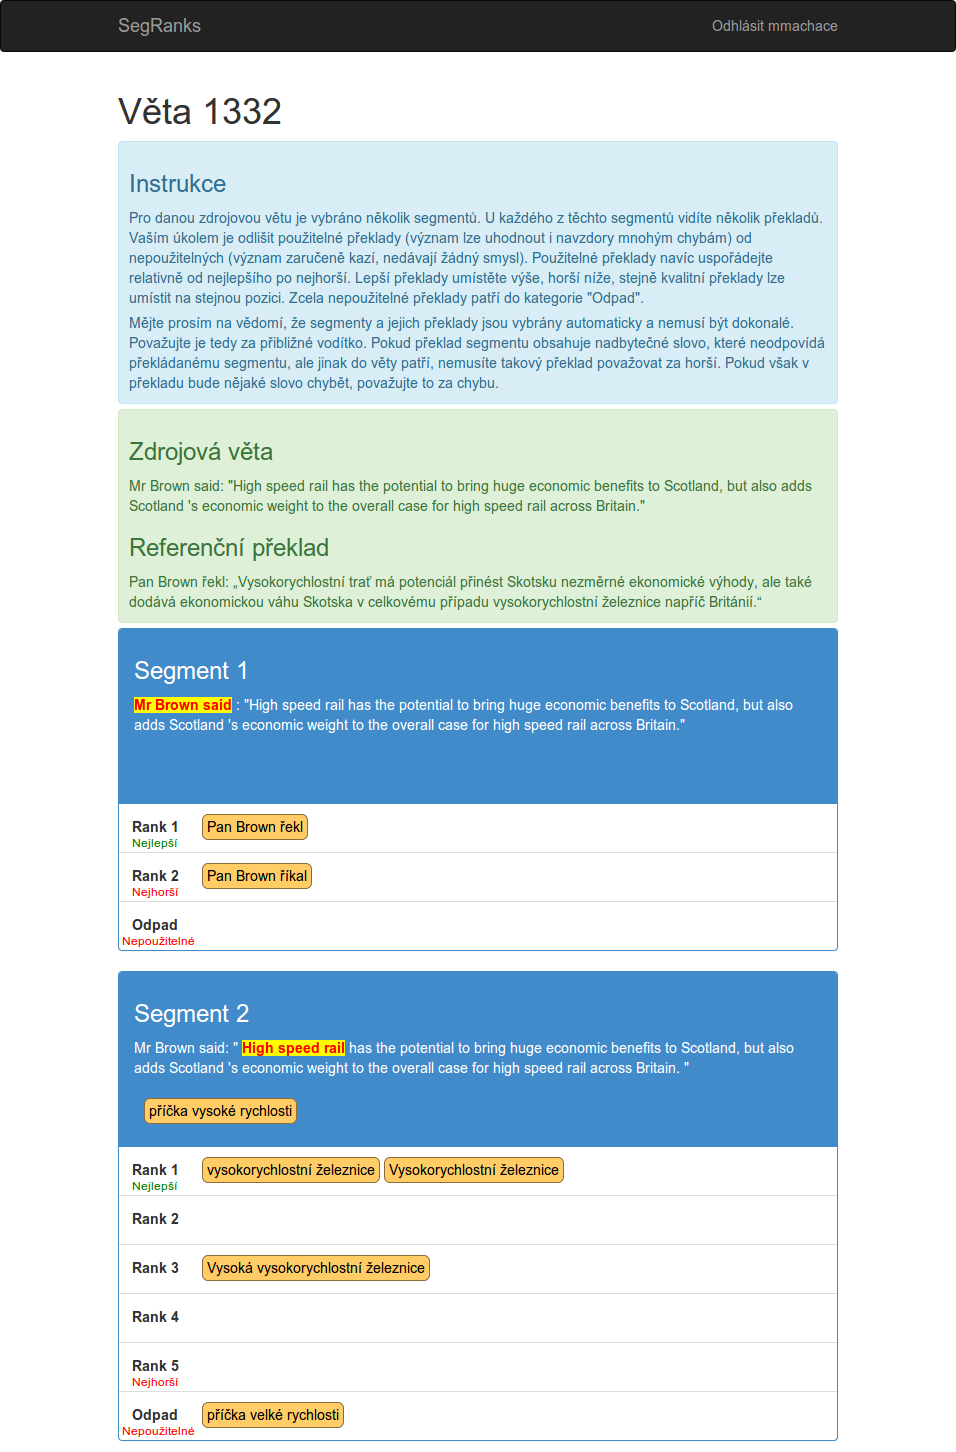
\includegraphics[width=\textwidth]{img/segranks-screenshot2.png}
    \end{center}
    \caption[A screenshot of the annotation application]{A screenshot of the
    annotation application. Annotators rank the candidate segments by dragging
and dropping them into the ranks.  Annotators see all annotated segments of a
sentence on a single screen.}
    \label{segranks-screenshot}
\end{figure}

\begin{quote}

A number of segments are extracted from the annotated sentence. You are shown a
few candidate translations for each of these segments. Your task is to
distinguish acceptable candidate translations (the meaning of the segment can
be guessed despite a few or more errors) from unacceptable ones (the meaning is
definitely not possible to guess from the candidate segment). Also please rank
the acceptable candidate translations relatively from the best ones to the
worst ones.  Please place better candidate translations higher and the worse
ones lower. You can place candidates of the same quality on the same rank.
We ask that you place unacceptable candidates to the position ``Garbage''

Please note that source segments and their candidate translations are chosen
automatically and do not have to be perfect. Consider them only as approximate
clues. If a candidate segment contains an extra word, which does not correspond
to the source segment but otherwise could be in the translated sentence, you do
not have to rank such candidate any worser. If something is missing in the
candidate translation you should consider it an error.

\end{quote}

Our goal was to make the annotation as efficient and user friendly as possible.
Annotators rank all the source segments of a sentence on a single screen (so
that they have to read the whole source sentence and reference translation only
once). For each annotated segment they see the source sentence repeated, with
the annotated segment highlighted. Annotators rank the segment candidates by
dragging and dropping them to appropriate rank positions. When all the
candidates of all the source segments of the sentence are ranked, annotators
are allowed to submit their annotations to the server.  The web interface has a
responsive design, so it is displayed correctly on smaller screens, and the
drag-and-drop works also on touch screens.  Annotators were therefore able to
rank segments on a tablet.


The very annotation experiment was conducted during May/June 2014 and it lasted
exactly one month. During this time, 17 annotators ranked segments of 2765
sentences, which is more than 92 \% of the prepared English-Czech test set.


\subsection{Annotator Agreements}

To measure the reliability and robustness of the proposed annotation method, we have
computed intra- and inter-annotator agreements. A reasonable degree of these
agreements supports the suitability of this method for machine translation
evaluation.

We measured the agreements using Cohen's kappa coefficient ($\kappa$)
\parcite{cohen1960}. Let $P(A)$ be the proportion of times the annotators agree
and $P(E)$ be the proportion of time that they would agree by chance. Then the
Cohen's $\kappa$ is computed using the following formula:

\begin{equation*}
    \kappa = \frac{P(A)-P(E)}{1-P(E)}
\end{equation*}

\noindent Simply put, $\kappa$ is the proportion of times the annotators agrees
of all the times they would not agree by chance. Note that $\kappa$ is a
normalized version of $P(A)$; it considers how difficult it is to agree without
knowing anything about the task.  Values of $\kappa$ can be therefore compared
in principle across various annotation experiments. The maximum value is 1
which would mean that annotators always agree.  A value of zero would mean that
annotators agree as often as they would by chance.

In our case, $P(A)$ and $P(E)$ are computed in the context of pairwise comparisons.
Approximately 5 \% of the annotated sentences were annotated twice by two
different annotators (for the inter-annotator agreement).  Another 5 \% of the
sentences were annotated twice by the same annotator (for the intra-annotator
agreement). From all the segments of these double annotated sentences, we
extracted pairwise comparisons of candidate segments. Then we computed $P(A)$
as the proportion of pairwise comparisons in which annotations match.

We computed the expected agreement by chance as 
\begin{equation*}
    P(E) = P(A>B)^2 + P(A=B)^2 + P(A<B)^2
\end{equation*}

\noindent where $P(A>B)$, $P(A=B)$ and $P(A<B)$ were computed empirically as
the relative frequencies of cases where the two segments $A$, $B$ are ranked
$>$, $=$, or $<$ respectively, across all annotations of the pair $A$, $B$,
regardless the sentence or annotator. The value of $P(E)$ in our experiment is
0.394, which means that the probability of the outcomes $A>B$, $A=B$ and $A<B$
is not uniform.

\begin{table}
    \begin{center}
        \begin{tabular}{r|cc}
                                     & our method & \cite{wmt14-overview-paper} \\
            \hline
            intra-annotator $\kappa$ &  0.593     & 0.448    \\
            inter-annotator $\kappa$ &  0.397     & 0.360     \\
        \end{tabular}
    \end{center}

    \caption[Inter-annotator and intra-annotator $\kappa$ scores]{$\kappa$
        scores measuring intra-annotator and inter-annotator agreements. We
        also report corresponding $\kappa$ scores from official WMT translation
        task for comparison.  Please see Table \ref{big-table} for the
    annotator agreements computed for individual annotators}

    \label{agreements}
\end{table}

The final values of inter-annotator and intra-annotator $\kappa$ can be found
in Table \ref{agreements} You can also compare them to the corresponding $\kappa$ values
from WMT14 translation task \parcite{wmt14-overview-paper}, which were computed similarly
on the same testset.  The exact interpretation of the Kappa
coefficient is difficult, but according to \cite{landis77}, 0 -- 0.2 is slight,
0.2 -- 0.4 is fair, 0.4 -- 0.6 is moderate, 0.6 -- 0.8 is substantial and 0.8
-- 1.0 is almost perfect.  You can see that we get both $\kappa$ scores better
than those of WMT14. However, they are still quite low and we expected them
to be higher, since the annotation task was designed to be much simpler than
the ranking full segments in the official WMT human evaluation.

We also computed the agreements $\kappa$ for individual annotators and report
them in Table \ref{big-table}.  As you can see, these scores are varying a lot.
Based on these scores, we could filter out unreliable annotators. However, we
do not do that in order to maintain comparability to the WMT14 experiment.


\begin{table}
    \begin{center}
        \begin{tabular}{|c|r|r|r|r|r|r|}
\hline
%\textbf{ID} & \rotatebox{90}{\textbf{\#sentences}} & \rotatebox{90}{\textbf{\#segments}} & \textbf{time} & \rotatebox{90}{\textbf{reward/CZK}} & \rotatebox{90}{\textbf{annotatin-time/seconds}} & \rotatebox{90}{\textbf{kappa-intra}} & \rotatebox{90}{\textbf{kappa-inter}} \\
ID & $n_{sent}$ & $n_{seg}$ & $t$ & $\frac{t}{n_{seg}}$ & $\kappa_{intra}$ & $\kappa_{inter}$ \\
\hline
1 & 78 & 232 & 4:53:43 &  75 & 0.838 & 0.495 \\
4 & 87 & 248 & 5:00:46 &  74 & 0.283 & 0.145 \\
6 & 378 & 1160 & 16:53:13 & 52 & 0.657 & 0.453 \\
7 & 243 & 663 & 11:16:26 &  62 & 0.763 & 0.417 \\
8 & 6 & 20 & 0:21:06 &  63 & & \\
9 & 12 & 50 & 0:45:58 &  55 & 0.686 & \\
10 & 98 & 274 & 5:04:45 &  66 & 0.673 & 0.320 \\
12 & 3 & 7 & 0:15:03 &  129 & 0.281 & \\
13 & 424 & 1260 & 1 day, 2:26:14 &  75 & 0.459 & 0.308 \\
15 & 106 & 282 & 5:17:58 &  67 & 0.611 & 0.401 \\
16 & 224 & 627 & 5:00:11 &  28 & 0.655 & 0.614 \\
17 & 26 & 74 & 2:40:44 &  130 & 0.734 & 0.269 \\
18 & 83 & 234 & 7:02:10 &  111 & 0.676 & 0.385 \\
19 & 15 & 50 & 1:31:52 &  110 & & \\
21 & 483 & 1443 & 1 day, 13:44:37 &  94 & 0.663 & 0.383 \\
22 & 117 & 338 & 6:00:36 &  64 & 0.714 & 0.431 \\
23 & 477 & 1371 & 22:07:35 &  58 & 0.376 & 0.363 \\
\hline
Total & 2773 & 8333 & 6 days, 14:22:57 &  68 & 0.593 & 0.397 \\
\hline
        \end{tabular}
    \end{center}

    \caption[A list of annotators and their statistics]{The list of annotators
      and their statistics. The annotators are anonymized using their ID. The
      table contains the number of annotated sentences $n_{sent}$, the number
      of annotated source segments $n_{seg}$ (this is not the number of ranked
      segment candidates), the time spent annotating $t$, the average time in
      seconds spent annotating one source segment $\frac{t}{n_{seg}}$, the
      normalized intra-annotator agreement $\kappa_{intra}$ and the normalized
      inter-annotator agreement $\kappa_{inter}$. }

    \label{big-table}
\end{table}


